\documentclass[12pt]{article}
\usepackage[top= 3cm, bottom=2cm, left=2cm, right=2cm]{geometry}
\usepackage[utf8]{inputenc}
\usepackage{url}
\usepackage{hyperref}
\hypersetup{
    colorlinks=true,
    urlcolor=blue,
    linkcolor=blue,
    citecolor=blue
    }
\usepackage{graphicx}
\usepackage[sorting=none]{biblatex} %Imports biblatex package
\addbibresource{biblio.bib} %Import the bibliography file

\usepackage[breakable]{tcolorbox}
\usepackage{enumerate}
\usepackage[spanish]{babel}
\usepackage{csquotes}
\usepackage{todonotes}

%SIMBOLOS
\usepackage{amsfonts} 
\usepackage{amsmath}
\usepackage{MnSymbol}
\usepackage{wasysym}
\usepackage{marvosym}

\usepackage{amsthm}
\setlength {\marginparwidth }{2cm}

%LISTINGS%%%%%%%%%%%%%%%%%%%%%%%%%%%%%%%%%%
\usepackage{multirow}
\usepackage{xcolor}
\usepackage{listings}
\usepackage{comment}
\usepackage{courier}
%LISTING JAVA%%%%%%%%%%%%%%%%%%%%%%%%%%%%%%%%%%
\definecolor{dkgreen}{rgb}{0,0.6,0}
\definecolor{gray}{rgb}{0.5,0.5,0.5}
\definecolor{mauve}{rgb}{0.58,0,0.82}
\definecolor{gray97}{gray}{.97}

%usando lstdefinestyle {java}{otrasconf} se pueden usar varias diferentes, luego para usarlo \begin{lstlisting}[style=java]
\lstdefinestyle{java}{frame=Ltb,
    language=Java,
    framerule=0pt,
    rulesep=.4pt,
    backgroundcolor=\color{gray97},
    rulesepcolor=\color{black},
    aboveskip=3mm,
    belowskip=3mm,
    showstringspaces=false,
    columns=flexible,
    basicstyle=\small\ttfamily,
    numbers=left,
    numberstyle=\tiny\color{gray},
    keywordstyle=\color{blue},
    commentstyle=\color{dkgreen},
    stringstyle=\ttfamily\color{black},
    breaklines=true,
    breakatwhitespace=true,
    tabsize=3
}
\usepackage{caption}
\DeclareCaptionFormat{listing}{\rule{\dimexpr\textwidth+0pt\relax}{0.4pt}\par\vskip1pt#1#2#3}
\captionsetup[lstlisting]{format=listing,singlelinecheck=false, margin=0pt, font={sf},labelsep=space,labelfont=bf}

\renewcommand\lstlistingname{Código}

\DeclareMathVersion{sans}
\SetSymbolFont{operators}{sans}{OT1}{cmbr}{m}{n}
\SetSymbolFont{letters}  {sans}{OML}{cmbrm}{m}{it}
\SetSymbolFont{symbols}  {sans}{OMS}{cmbrs}{m}{n}

\lstnewenvironment{sflisting}[1][]
  {\lstset{#1}\mathversion{sans}}{}
%%%%%%%%%%%%%%%%%%%%%%%%%%%%%%%%%%%%%%%%%%%%
\usepackage{fancyhdr}
\pagestyle{fancy}

%%%COMPLETAR%%% 
\fancyhead[L]{Trabajo Práctico NOMBRE}
\fancyhead[R]{NOMBRE MATERIA}



\begin{document}
\begin{titlepage}
  \title{\textbf{NOMBRE MATERIA}\\
  %\vspace{2mm}
  \large{\textbf{TITULO PRACTICO}}
  %\vspace{3mm}
  \author{
  Manuel Latorre FAI-1931\\ manuel.latorre@est.fi.uncoma.edu.ar\vspace{3mm}\\
  }}
  \date{Segundo cuatrimestre 2023}

  \pagenumbering{gobble}
  \maketitle
  \vspace{25mm}
  \vfill
  \hspace*{-0.1in}{
  
\includegraphics[width=7cm, scale=0.5]{Images/Unco/faiLogo.png}
  \hspace*{1.5in}
  
\includegraphics[width=5cm, scale=0.5]{Images/Unco/Unco logo.png}
  }
\end{titlepage}

\titlepage

\newpage

\pagebreak

%INDICE Y FIGURAS
\newpage
\tableofcontents %%Indice
\listoffigures
\clearpage\pagenumbering{arabic}
\newpage

%INPUTS
\section{Introducción}
En el presente informe se desarrollará el proceso de implementación de una aplicación Android con React Native. Dicha aplicación busca la carga y visualización de recetas de cocina, permitiendo a usuarios registrarse e iniciar sesión para poder subir, calificar y marcar como favoritas sus propias recetas. Se hará uso de una RESTful API para, desde el cliente, poder obtener toda la información relativa a las recetas. Las principales tecnologías utilizadas para el desarrollo del cliente son React Native para el desarrollo de la interfaz gráfica, Redux para el manejo de estados y Cloud Storage for Firebase para el almacenamiento y recuperación de imágenes. Las tecnologías utilizadas para la API son JavaScript, Node.js, Express.js y MySQL entre otras.
\subsection{RESTful API}
La RESTful API fue diseñada en primera instancia durante el cursado de la materia Laboratorio de programación utilizando JavaScript, Node.js y Express.js. Para la implementación de este trabajo se realizo una nueva API usando las mismas tecnologías y tomando como base la anterior mencionada con el fin de mejorar aspectos organizativos y funcionales.

Ademas con el fin de tener información persistente se agrego una base de datos mySQL para el almacenamiento de la información, considerando que las imágenes a utilizar iban a ser cargadas en un almacenamiento en la nube por lo que solo es necesario almacenar el enlace a estas para poder accederlas luego.

\begin{figure}[!h]
  \centering
  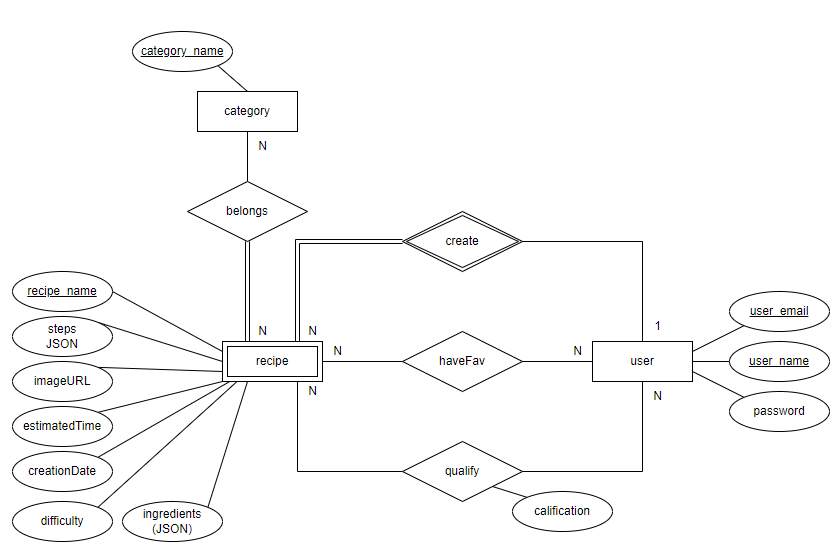
\includegraphics[width=16cm, scale=1]{Images/Imagenes/MER.png}
  \caption{Modelo entidad relación de la base de datos implementada}
  \label{fig:marcado}
\end{figure}

La implementación cuenta con método de población de la base de datos que puede ser ejecutado con el comando  \texttt{npm run populate}. Este se encargara de cargar con usuarios, recetas, categorías y favoritos a la base de datos para agilizar su prueba.

\subsection{Patrón MVC}
Como patron de diseño para la implementacion se utilizo Model View Controller (MVC). Este consiste en las siguientes capas:
\begin{itemize}
  \item \textbf{El modelo: }Representa los datos y la lógica de negocio de la aplicación. En el caso de esta implementación se corresponde con la capa de servicios que se encarga de realizar las consultas a la base de datos de forma directa. Puede encontrarse en el directorio \texttt{/services}
  \item \textbf{La vista: }Es la capa de presentación de la aplicación, que se encarga de mostrar los datos al usuario. En el contexto de una API RESTful, esta capa se corresponde con las respuestas que envía el servidor a las peticiones realizadas por los clientes. Puede encontrarse en el directorio \texttt{/routes}
  \item \textbf{El controlador: }es la capa que se encarga de manejar las peticiones del usuario, interactuar con el modelo para obtener los datos necesarios y devolver la respuesta adecuada. En este caso se utilizaron rutas y controladores que reciben peticiones, validan los datos y solicitan informacion a los servicios correspondientes. Puede encontrarse en los directorios \texttt{/controllers} y \texttt{/middlewares/validators}
\end{itemize}

\subsection{Ejecución Otras consideraciones}
Una vez configurado el .env de manera adecuada la API puede ponerse en marcha con el comando \texttt{npm run dev}.

Otras bibliotecas importantes para la implementación de la api son:

\begin{itemize}
  \item \textbf{Bcrypt: }Para realizar el cifrado de las contraseñas de los usuarios
  \item \textbf{Dotenv: }Para definir variables de entorno y facilitar asi la configuración de la API y la base de datos. Es conveniente revisar dicho archivo para configurar adecuadamente la API e iniciar la ejecución.  
  \item \textbf{JSON Web Token (JWT): }como mecanismo de autenticación y autorización con los clientes
\end{itemize}

Para el realizar pruebas se hizo uso de Postman, en la figura [\ref{fig:postman}] se puede observar la lista de pruebas realizadas las cuales también se corresponden con los diferentes servicios que brinda la API.

\begin{figure}[!htb]
  \centering
  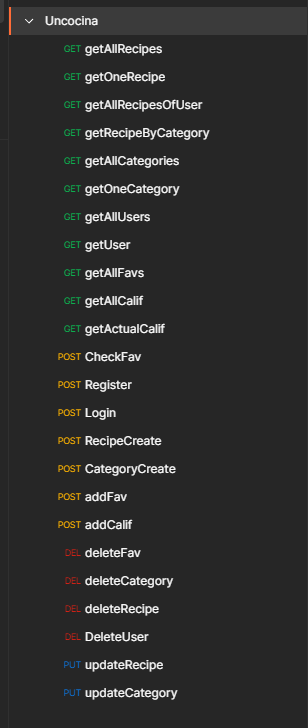
\includegraphics[width=8cm, scale=1]{Images/Imagenes/postman.png}
  \caption{Lista de pruebas realizadas a la API con Postman}
  \label{fig:postman}
\end{figure}


\newpage
\section{Cliente}
El cliente fue implementado con React Native utilizando la herramienta Expo. Este se sirve de información provista por la API a traves de peticiones realizadas con Axios. 

\subsection{Patron Flux}
Se opto por un patron Flux para el desarrollo debido a su conveniencia para la implementación de aplicaciones que manejan grandes cantidades de datos o que necesitan ser actualizadas en tiempo real.

El patrón Flux consta de cuatro elementos principales: el Store, el Dispatcher, las Actions y la View. La Store es una especie de base de datos en la que se almacenan los datos de la aplicación (para esto se utilizo Redux Toolkit). El Dispatcher es el encargado de recibir y distribuir las acciones que se realizan en la aplicación. Las Actions son objetos que describen una acción específica que se realizará en la aplicación, y la View es la interfaz de usuario que se muestra al usuario.

El patrón Flux utiliza un flujo de datos unidireccional, lo que significa que la información se mueve en una dirección desde las Actions hasta la View. Cuando un usuario realiza una acción en la aplicación, se crea un objeto Action que describe la acción que se ha realizado. El Dispatcher recibe esta acción y la distribuye a la Store, donde se actualiza el estado de la aplicación. Finalmente, la View se actualiza para reflejar el estado actual de la aplicación.



\subsection{Las vistas}

\textbf{Vista de inicio de sesión: }
Permite el inicio de sesión por parte de los usuarios con un email y contraseña. Realiza una validación en caso de que falte ingresar algún dato, el email no se encuentre registrado o la contraseña no sea valida. Figura \ref{fig:login1} y Figura \ref{fig:login2}\\

\begin{figure}[!h]
  \centering
  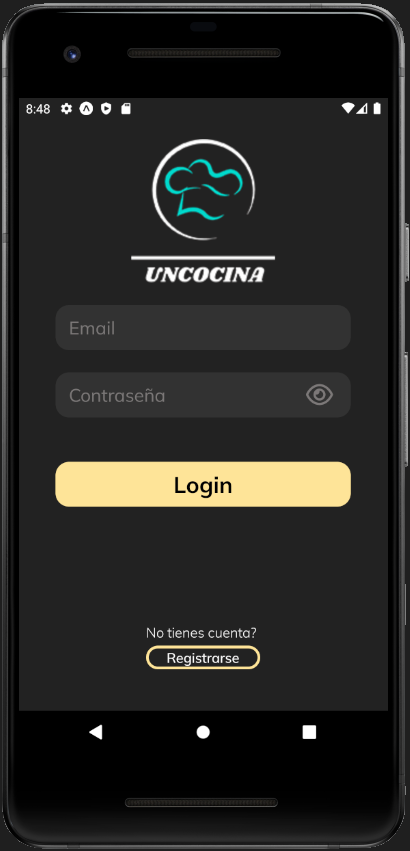
\includegraphics[width=8cm, scale=1]{Images/Imagenes/login1.png}
  \caption{Vista de inicio de sesión}
  \label{fig:login1}
\end{figure}

\begin{figure}[!h]
  \centering
  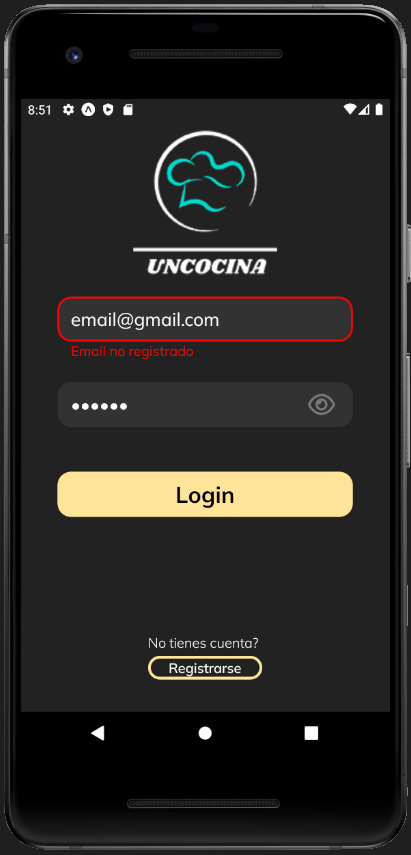
\includegraphics[width=8cm, scale=1]{Images/Imagenes/login2.png}
  \caption{Vista de inicio de sesión con validación}
  \label{fig:login2}
\end{figure}

\textbf{Vista de registro: }
Permite el registro de usuarios a la plataforma. Realiza el mismo tipo de validaciones que la pantalla de inicio de sesión. Figura \ref{fig:registro}\\

\begin{figure}[!h]
  \centering
  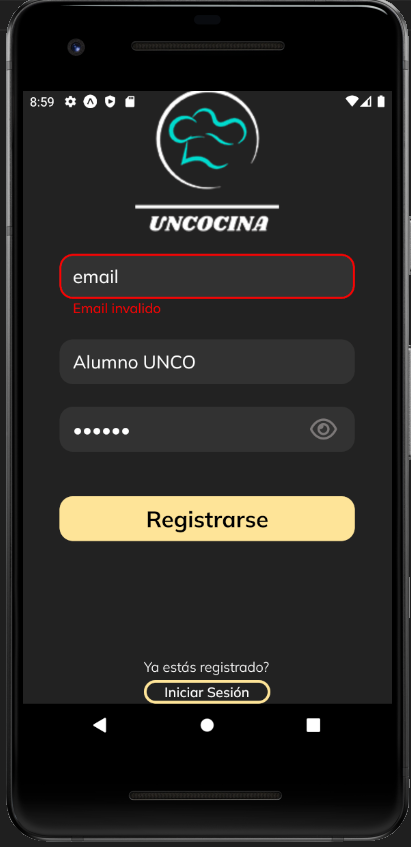
\includegraphics[width=8cm, scale=1]{Images/Imagenes/registro.png}
  \caption{Vista de registro}
  \label{fig:registro}
\end{figure}

\textbf{Vista de recetas: }
Una vez el usuario se registra o inicia sesión es redireccionado automáticamente a esta vista, aquí se mostrara todas las recetas de la base de datos permitiendo ordenarlas por fecha de publicación y filtrar por categorías. Ademas como la API soporta paginación las recetas se van cargando a medida que se ``scrollea'' hacia abajo. Figura \ref{fig:recetas1}, Figura \ref{fig:recetas2} y Figura \ref{fig:recetas3}\\

\begin{figure}[!h]
  \centering
  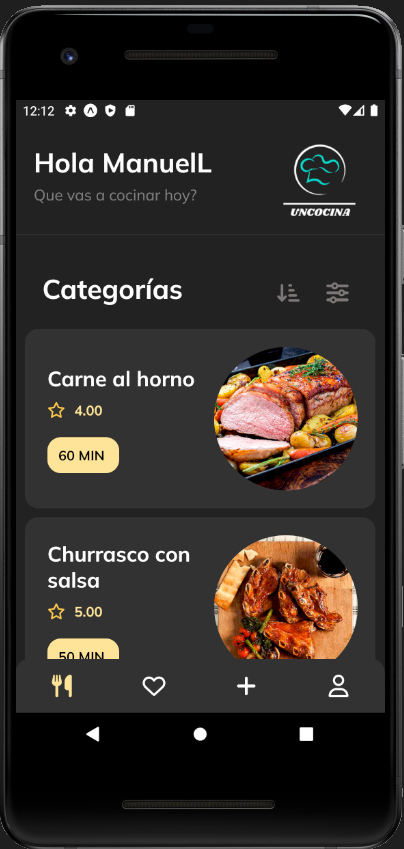
\includegraphics[width=8cm, scale=1]{Images/Imagenes/recetas1.png}
  \caption{Vista de recetas}
  \label{fig:recetas1}
\end{figure}

\begin{figure}[!h]
  \centering
  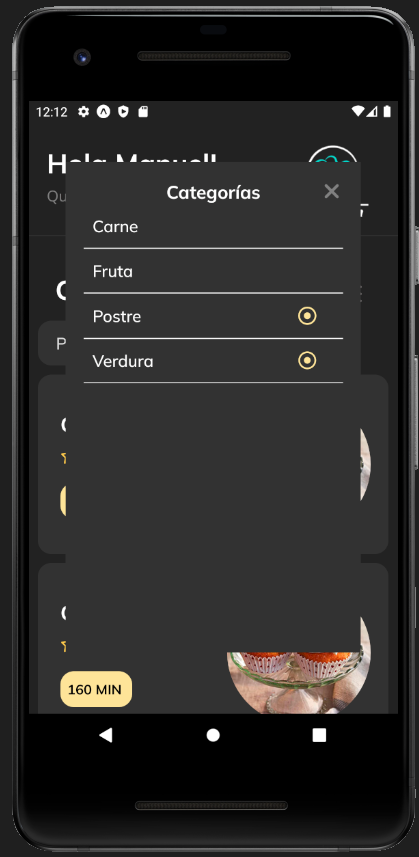
\includegraphics[width=8cm, scale=1]{Images/Imagenes/recetas2.png}
  \caption{Selección de categorías para filtrar}
  \label{fig:recetas2}
\end{figure}

\begin{figure}[!h]
  \centering
  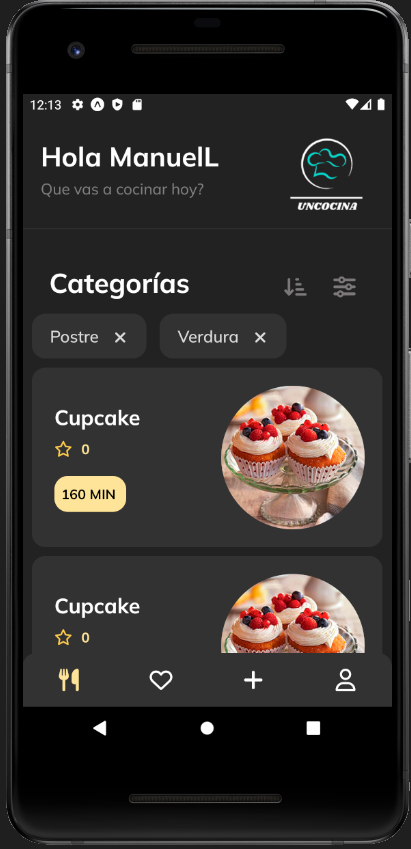
\includegraphics[width=8cm, scale=1]{Images/Imagenes/recetas3.png}
  \caption{Vista de recetas con categorías filtradas}
  \label{fig:recetas3}
\end{figure}

\textbf{Vista de favoritos: }
Esta vista reutiliza el componente utilizado para la vista de recetas para mostrar las recetas seleccionadas como favoritas por los usuarios. Puede accederse a traves del navbar ubicado en la parte baja de la pantalla. Figura \ref{fig:favoritos} y Figura \ref{fig:favoritos2}\\

\begin{figure}[!h]
  \centering
  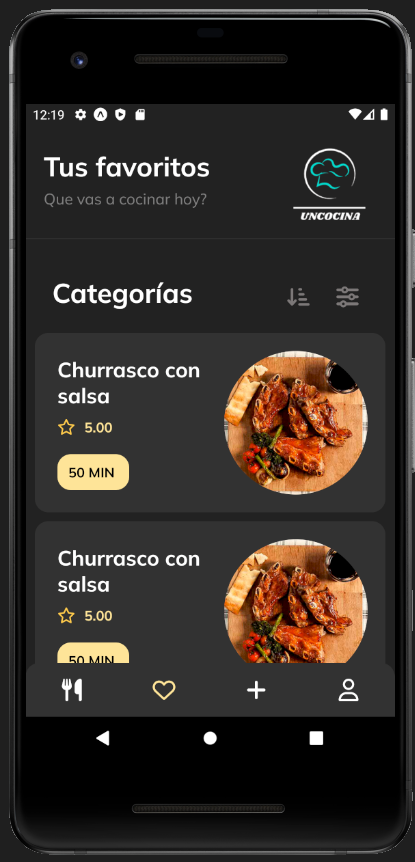
\includegraphics[width=8cm, scale=1]{Images/Imagenes/favoritos.png}
  \caption{Vista de favoritos}
  \label{fig:favoritos}
\end{figure}

\begin{figure}[!h]
  \centering
  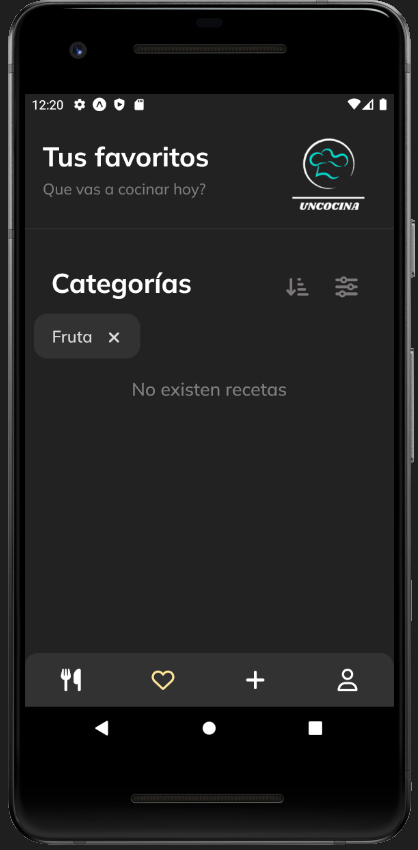
\includegraphics[width=8cm, scale=1]{Images/Imagenes/favoritos2.png}
  \caption{Vista de favoritos con una categoría de recetas seleccionada para la cual aun no existen favoritos}
  \label{fig:favoritos2}
\end{figure}

\textbf{Vista información de receta: }
Si en las vistas de recetas o favoritos se presiona sobre alguna de las recetas se llegara a la vista de información de dicha receta. Aquí se pueden ver listados los pasos de la receta, ingredientes, duración, imagen, se puede realizar una calificación sobre la receta y agregarla a favoritos. Ademas se utilizo el componente externo ``\texttt{@gorhom/bottom-sheet}'' para poner los ingredientes en un cajon deslizable. Figura \ref{fig:inforeceta1}, Figura \ref{fig:inforeceta2}, Figura \ref{fig:inforeceta3} y Figura \ref{fig:inforeceta4}\\

\begin{figure}[!h]
  \centering
  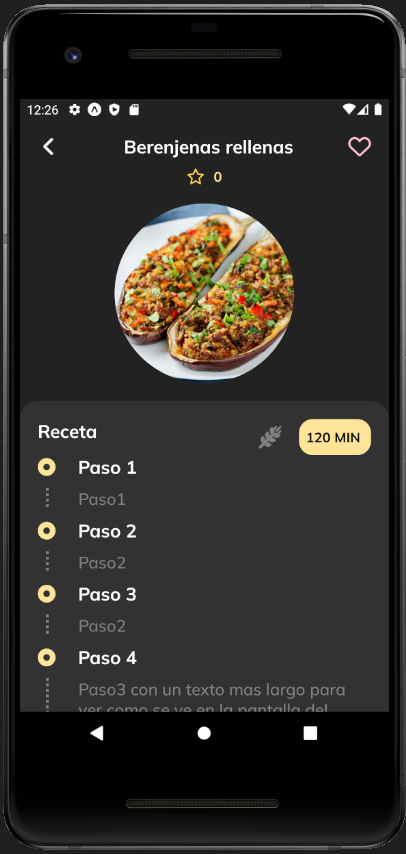
\includegraphics[width=8cm, scale=1]{Images/Imagenes/inforeceta1.png}
  \caption{Vista de información de receta}
  \label{fig:inforeceta1}
\end{figure}

\begin{figure}[!h]
  \centering
  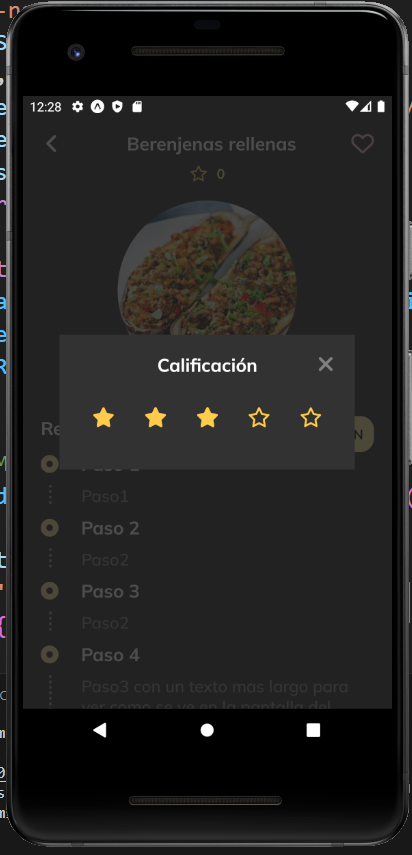
\includegraphics[width=8cm, scale=1]{Images/Imagenes/inforeceta2.png}
  \caption{Vista de calificación de receta}
  \label{fig:inforeceta2}
\end{figure}

\begin{figure}[!h]
  \centering
  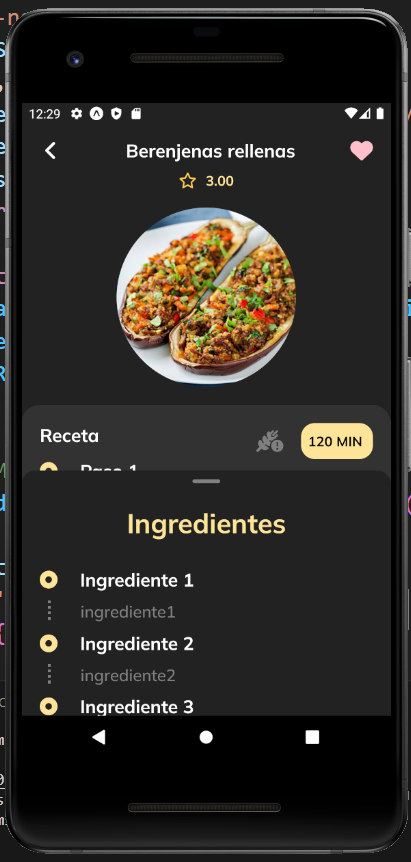
\includegraphics[width=8cm, scale=1]{Images/Imagenes/inforeceta3.png}
  \caption{Vista de información de receta con cajon de ingredientes a mitad de pantalla}
  \label{fig:inforeceta3}
\end{figure}

\begin{figure}[!h]
  \centering
  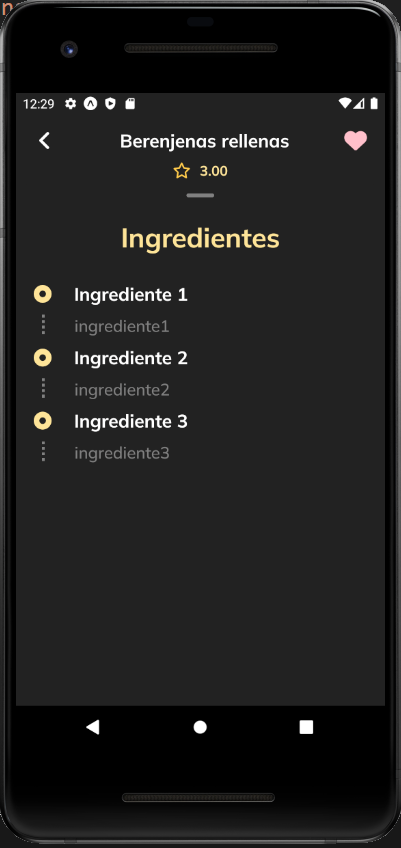
\includegraphics[width=8cm, scale=1]{Images/Imagenes/inforeceta4.png}
  \caption{Vista de calificación información de receta con cajon de ingredientes completamente abierto}
  \label{fig:inforeceta4}
\end{figure}

\textbf{Vista de creación de receta: }
En esta vista se solicitaran todos los datos necesarios para crear una nueva receta. Se realizaran las validaciones correspondientes y una vez cargada la receta exitosamente ser redireccionara a la vista de recetas donde se podrá ver publicada. Figuras [\ref{fig:add1}],[\ref{fig:add2}],[\ref{fig:add3}],[\ref{fig:add4}],[\ref{fig:add5}],[\ref{fig:add6}],[\ref{fig:add7}],[\ref{fig:add8}],[\ref{fig:add9}]\\

\begin{figure}[!h]
  \centering
  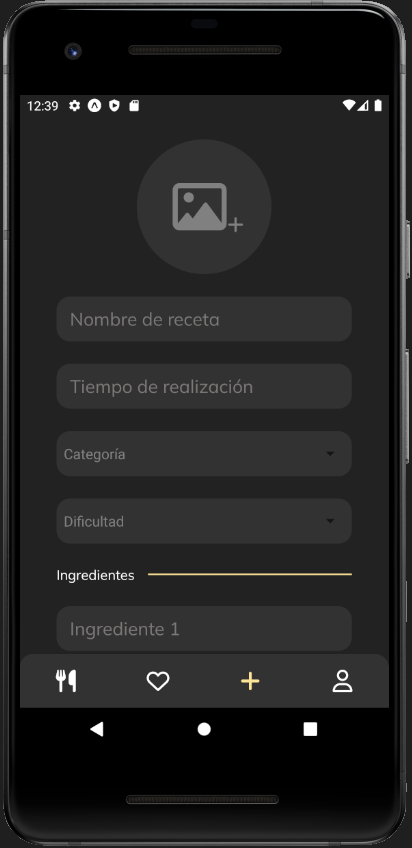
\includegraphics[width=8cm, scale=1]{Images/Imagenes/add1.png}
  \caption{Vista de creación de receta}
  \label{fig:add1}
\end{figure}

\begin{figure}[!h]
  \centering
  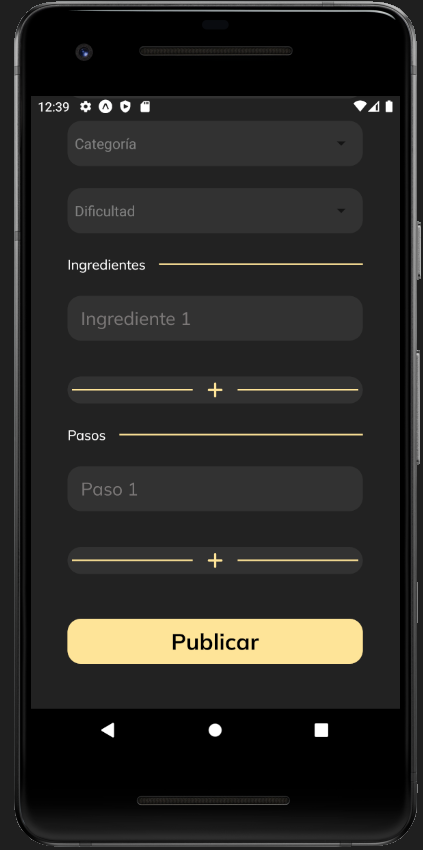
\includegraphics[width=8cm, scale=1]{Images/Imagenes/add2.png}
  \caption{Vista de creación de receta}
  \label{fig:add2}
\end{figure}

\begin{figure}[!h]
  \centering
  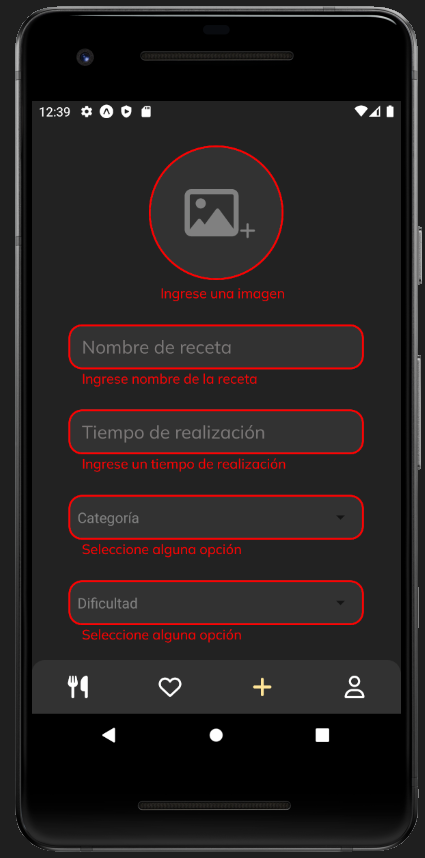
\includegraphics[width=8cm, scale=1]{Images/Imagenes/add3.png}
  \caption{Vista de creación de receta con validaciones}
  \label{fig:add3}
\end{figure}

\begin{figure}[!h]
  \centering
  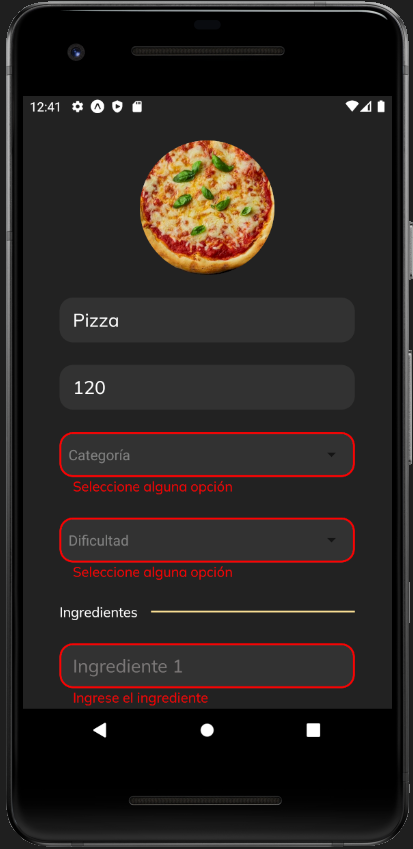
\includegraphics[width=8cm, scale=1]{Images/Imagenes/add4.png}
  \caption{Vista de creación de receta}
  \label{fig:add4}
\end{figure}

\begin{figure}[!h]
  \centering
  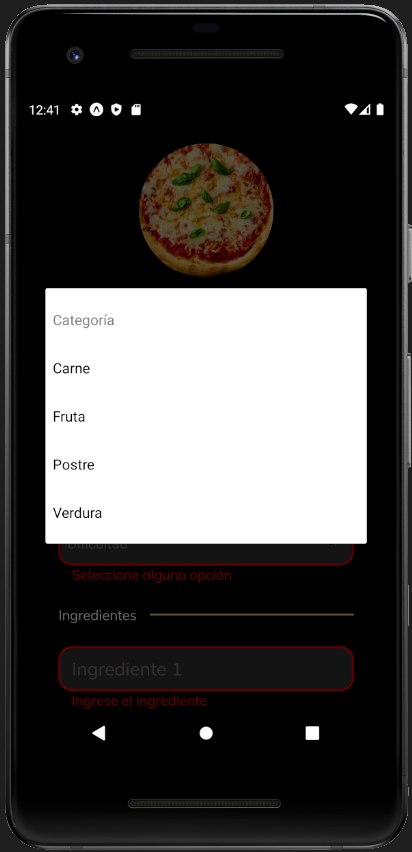
\includegraphics[width=8cm, scale=1]{Images/Imagenes/add5.png}
  \caption{Vista de creación de receta seleccionando la categoría}
  \label{fig:add5}
\end{figure}

\begin{figure}[!h]
  \centering
  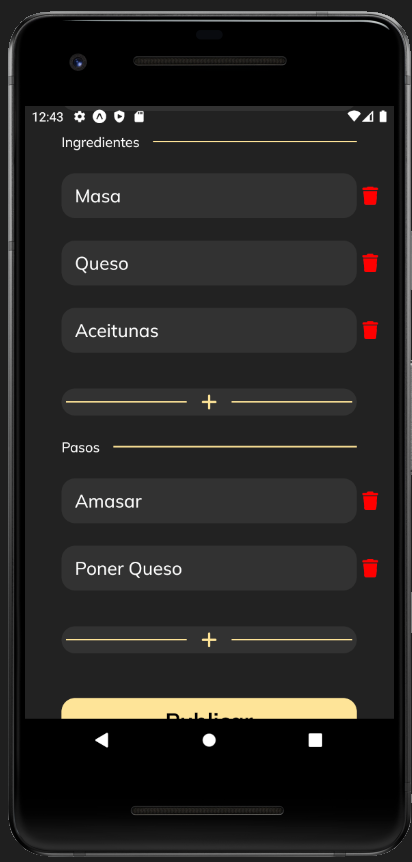
\includegraphics[width=8cm, scale=1]{Images/Imagenes/add6.png}
  \caption{Vista de creación de receta definiendo los ingredientes y pasos a seguir}
  \label{fig:add6}
\end{figure}

\begin{figure}[!h]
  \centering
  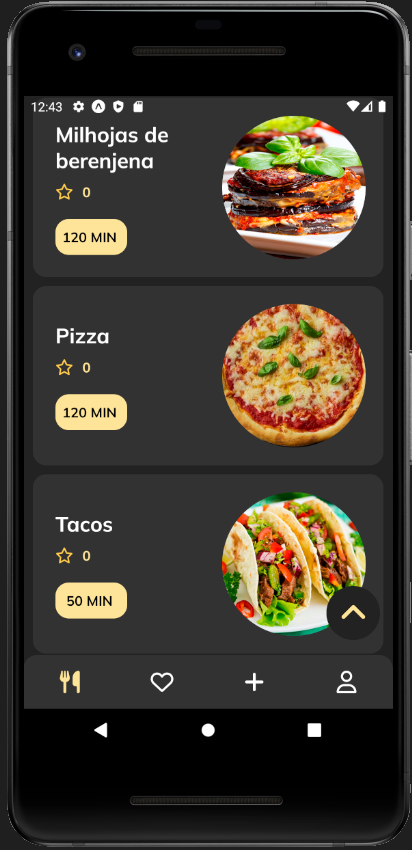
\includegraphics[width=8cm, scale=1]{Images/Imagenes/add7.png}
  \caption{Vista recetas en donde se ve la nueva receta agregada}
  \label{fig:add7}
\end{figure}

\begin{figure}[!h]
  \centering
  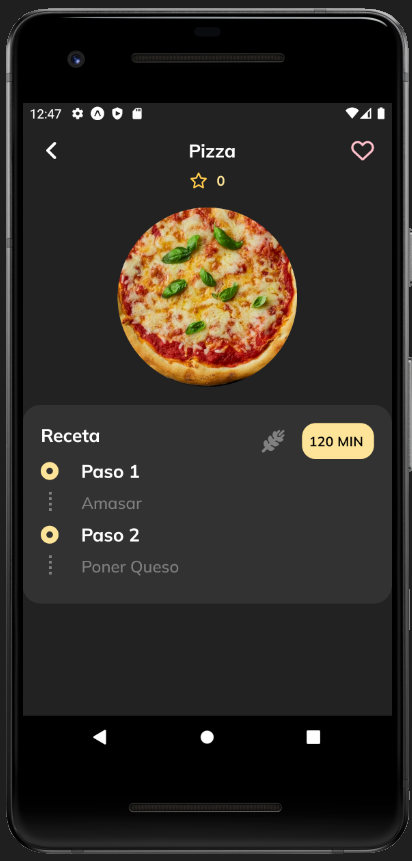
\includegraphics[width=8cm, scale=1]{Images/Imagenes/add8.png}
  \caption{Vista información de la receta creada}
  \label{fig:add8}
\end{figure}

\begin{figure}[!h]
  \centering
  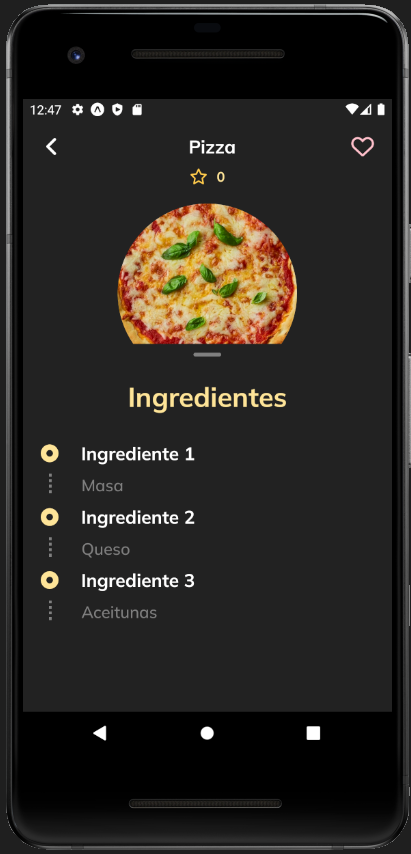
\includegraphics[width=8cm, scale=1]{Images/Imagenes/add9.png}
  \caption{Vista información de la receta creada}
  \label{fig:add9}
\end{figure}

\textbf{Vista de cierre de sesión: }
Finalmente se cuenta con una vista para cerrar la sesión, al hacerlo redirecciona automáticamente a la vista de inicio de sesión. Figura \ref{fig:cierre}

\begin{figure}[!h]
  \centering
  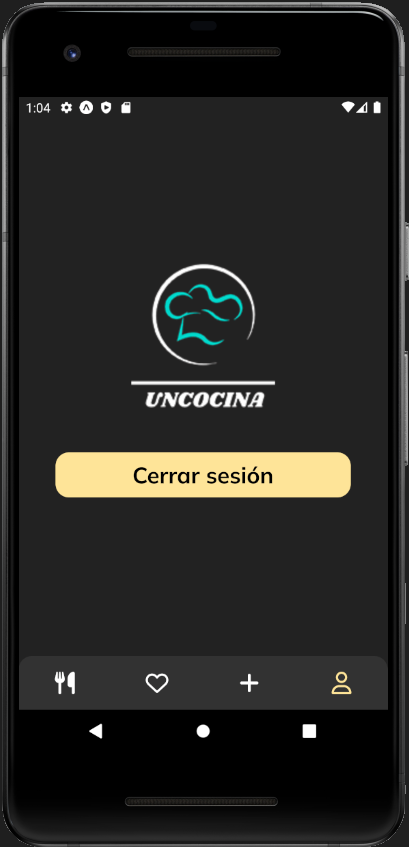
\includegraphics[width=8cm, scale=1]{Images/Imagenes/cierre.png}
  \caption{Vista cierre de sesión}
  \label{fig:cierre}
\end{figure}

\printbibliography
\end{document}